\documentclass[aspectratio=169]{beamer}

% ==================================================================
% Define custom colors
\definecolor{primarycolor}{RGB}{25, 74, 166} % blue
\definecolor{accentcolor}{RGB}{65, 155, 232} % lighter blue
\definecolor{bluepoli}{RGB}{2, 30, 54}
\newcommand{\highlight}[2]{\colorbox{#1!9}{$#2$}}

% ==================================================================
% Apply these colors
\setbeamercolor{normal text}{fg=black, bg=white}
\setbeamercolor{alerted text}{fg=accentcolor}
\setbeamercolor{example text}{fg=accentcolor!80!black}
\setbeamercolor{progress bar}{fg=accentcolor, bg=accentcolor!20}
\setbeamercolor{frametitle}{bg=bluepoli, fg=bluepoli!80!black}
\setbeamercolor{title separator}{fg=bluepoli}

% ==================================================================
% Metropolis customization
\usetheme[sectionpage=none]{metropolis}
\setbeamercolor{background canvas}{bg=black!1.5}
\setbeamercolor{frametitle}{bg=black!1.5,fg=black}
\setbeamertemplate{sections/subsections in toc}[square]
\setbeamertemplate{footline}{
    \centerline{\textcolor{bluepoli}{\rule{0.95\paperwidth}{.3pt}}}
    \vskip2.5pt
    \hskip15pt \tiny Linear system of equations \hskip330pt \insertframenumber
    \vskip4pt
}

% ==================================================================
% Images
\usepackage{graphicx}

% ==================================================================
% Colors
\usepackage{color}
\usepackage[dvipsnames]{xcolor}
\usepackage{colortbl}

% ==================================================================
% Code rendering
\usepackage{minted}

% ==================================================================
% TIKZ
\usepackage{tikz}
\usetikzlibrary{positioning,tikzmark,backgrounds,arrows,shapes,calc}

% ==================================================================
% TITLE
\title{Linear System Of Equations\\Part 1}
\subtitle{Calcoli di Processo dell' Ingegneria Chimica}
\author[Dinelli]{\textbf{Timoteo~Dinelli}}
\institute{
   \inst{} Department of Chemistry, Materials and Chemical Engineering, ``Giulio Natta'', Politecnico di Milano.\\ \\
   \textbf{email}: timoteo.dinelli@polimi.it
}
\date{9\textsuperscript{th} of October 2025}

\begin{document}
{
\setbeamertemplate{footline}{}
\begin{frame}{}
	\maketitle
	\begin{tikzpicture}[overlay, remember picture]
		\node[above left=3.6cm and 0.01cm of current page.south east]{
\includegraphics[trim=1cm 1cm 5.5cm 1cm, clip=true, width=8cm]{figures/logo.pdf}};
	\end{tikzpicture}
\end{frame}
}

% ==================================================================
% Slides
\begin{frame}{Motivation: Why Linear Systems?}
	\small{
		Consider a chemical process with multiple unit operations. Mass balance equations for each component form a system of equations:
	}
	\vspace{0.3cm}

	% \begin{equation*}
	%     \begin{cases}
	%         \text{Reactor: } \quad 2x_1 + x_2 - x_3 = 100 \\
	%         \text{Separator: } \quad x_1 + 3x_2 + x_3 = 150 \\
	%         \text{Mixer: } \quad -x_1 + x_2 + 4x_3 = 200
	%     \end{cases}
	% \end{equation*}
	\begin{columns}
		\column{0.7\textwidth}
		\begin{figure}
			\centering
			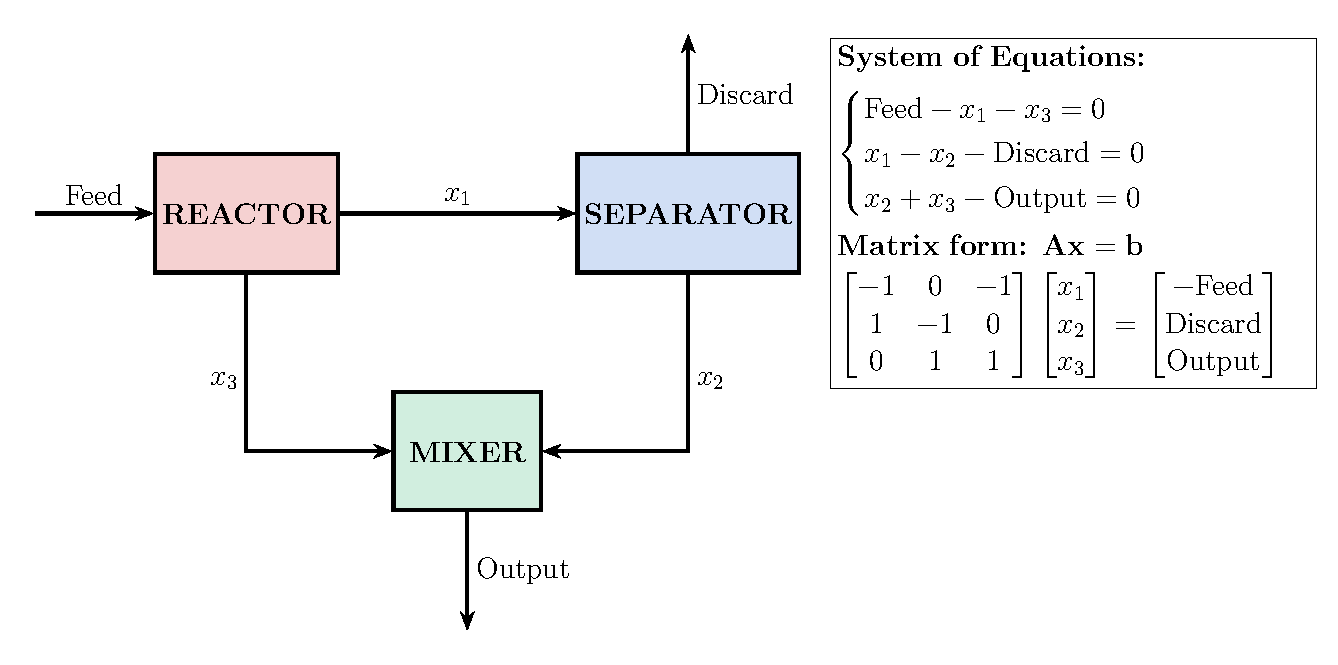
\includegraphics[width=\textwidth]{figures/process.pdf}
		\end{figure}

		\column{0.3\textwidth}
		\footnotesize{Where $x_1, x_2, x_3$ represent flow rates. Such systems appear everywhere in engineering: heat transfer, electrical circuits, structural analysis, and process optimization.}
	\end{columns}

	\vspace{0.1cm}
	\alert{How do we solve these efficiently and accurately?}
\end{frame}

\begin{frame}{Linear System Of Equations}
	\small{
		A system of linear equations consists of several \alert{linear equations} that must all be satisfied simultaneously. A solution is a vector whose elements, when substituted for the unknowns, satisfy all equations.
	}

	From the classical representation to the \alert{\textbf{matrix}} form:
	\begin{columns}
		\column{0.5\textwidth}
		\begin{equation*}
			\begin{cases}
				a_{1,1}x_{1} + a_{1,2}x_{2} + \ldots + a_{1,n}x_{n} = b_{1} \\
				a_{2,1}x_{1} + a_{2,2}x_{2} + \ldots + a_{2,n}x_{n} = b_{2} \\
				\quad \quad \vdots                                          \\
				a_{n,1}x_{1} + a_{n,2}x_{2} + \ldots + a_{n,n}x_{n} = b_{n}
			\end{cases}
		\end{equation*}

		\column{0.5\textwidth}
		\begin{equation*}
			\tikzmarknode{Amatrix}{\highlight{OliveGreen}{
					\begin{bmatrix}
						a_{1,1} & a_{1,2} & \ldots & a_{1,n} \\
						a_{2,1} & a_{2,2} & \ldots & a_{2,n} \\
						\vdots  & \vdots  & \ddots & \vdots  \\
						a_{n,1} & a_{n,2} & \ldots & a_{n,n}
					\end{bmatrix}
				}}\:
			\tikzmarknode{xvector}{\highlight{NavyBlue}{
					\begin{bmatrix}
						x_{1}  \\
						x_{2}  \\
						\vdots \\
						x_{n}
					\end{bmatrix}
				}}
			=
			\tikzmarknode{bvector}{\highlight{WildStrawberry}{
					\begin{bmatrix}
						b_{1}  \\
						b_{2}  \\
						\vdots \\
						b_{n}
					\end{bmatrix}
				}}
		\end{equation*}
	\end{columns}

	\begin{equation*}
		\textcolor{OliveGreen}{\mathbf{A}} \: \textcolor{NavyBlue}{\mathbf{x}} = \textcolor{WildStrawberry}{\mathbf{b}}
	\end{equation*}
\end{frame}

\begin{frame}{Why Not Just Invert the Matrix?}
	The ``obvious'' solution would be:
	\begin{equation*}
		\mathbf{x} = \mathbf{A}^{-1} \mathbf{b}
	\end{equation*}

	\textcolor{WildStrawberry}{\textbf{This approach is impractical!}} Here's why:
	\vspace{0.1cm}

	\begin{itemize}
		\item[$\blacktriangleright$]
		      \textbf{Computational cost:} Computing $\mathbf{A}^{-1}$ requires $\sim O(n^3)$ operations, same as solving the system directly
		      \vspace{0.3cm}
		\item[$\blacktriangleright$]
		      \textbf{Numerical instability:} Direct inversion amplifies rounding errors, especially for ill-conditioned matrices
		      \vspace{0.3cm}
		\item[$\blacktriangleright$]
		      \textbf{Memory:} Storing the full inverse matrix requires $n^2$ memory locations
		      \vspace{0.3cm}
		\item[$\blacktriangleright$]
		      \textbf{Singularity:} If $\det(\mathbf{A}) = 0$, the inverse doesn't exist
	\end{itemize}
\end{frame}

\begin{frame}{The Goal: Triangular Systems}
	\noindent Consider this simple $3 \times 3$ \alert{upper triangular} system:
	\vspace{0.5cm}

	\begin{columns}
		\column{0.5\textwidth}
		\begin{equation*}
			\begin{cases}
				3x + 89y + 66z = 87 \\
				65y + 9z = 7        \\
				46z = 3
			\end{cases}
		\end{equation*}
		\column{0.5\textwidth}
		\begin{equation*}
			\begin{bmatrix}
				3 & 89 & 66 \\
				0 & 65 & 9  \\
				0 & 0  & 46
			\end{bmatrix}
			\begin{bmatrix}
				x \\ y \\ z
			\end{bmatrix} =
			\begin{bmatrix}
				87 \\ 7 \\ 3
			\end{bmatrix}
		\end{equation*}
	\end{columns}

	\vspace{0.3cm}
	\begin{columns}
		\column{0.5\textwidth}
		\small{This is \textbf{easy to solve} by \alert{back-substitution}}:
		\begin{align*}
			z & = \frac{3}{46} \approx 0.065             \\
			y & = \frac{7 - 9z}{65} \approx 0.098        \\
			x & = \frac{87 - 89y - 66z}{3} \approx 26.09
		\end{align*}
		\column{0.5\textwidth}
		Cost: Only $O(n^2)$ operations!\\
		\textcolor{WildStrawberry}{\textbf{Our goal: Transform any system into triangular form.}}
	\end{columns}
\end{frame}

% \begin{frame}{Example: Gauss Elimination Step-by-Step}
%     Let's solve a simple $2 \times 2$ system to see the mechanics:
%     \begin{equation*}
%         \begin{cases}
%             2x + 3y = 8 \\
%             4x + 5y = 14
%         \end{cases}
%     \end{equation*}
%     
%     \begin{columns}
%     \column{0.5\textwidth}
%         \textbf{Step 1:} Form augmented matrix
%         \begin{equation*}
%             \left[\begin{array}{cc|c}
%                 2 & 3 & 8 \\
%                 4 & 5 & 14
%             \end{array}\right]
%         \end{equation*}
%     
%     \column{0.5\textwidth}
%         \textbf{Step 2:} Eliminate $a_{2,1}$ using multiplier $m_{2,1} = \frac{a_{2,1}}{a_{1,1}} = \frac{4}{2} = 2$
%     
%         Row 2 $\leftarrow$ Row 2 $- 2 \times$ Row 1:
%         \begin{equation*}
%             \left[\begin{array}{cc|c}
%                 2 & 3 & 8 \\
%                 0 & -1 & -2
%             \end{array}\right]
%         \end{equation*}
%     \end{columns}
%     
%     \textbf{Step 3:} Back-substitution: $y = 2$, then $x = 1$
% \end{frame}

\begin{frame}{Gauss Elimination: General Algorithm}
	\small{Given $\mathbf{A}\mathbf{x} = \mathbf{b}$, form the \alert{augmented matrix} $\mathbf{A}^{*} = [\mathbf{A} \, | \, \mathbf{b}]$}
	\vspace{0.15cm}
	\begin{equation*}
		\mathbf{A}^{*} = [\mathbf{A} \, | \, \mathbf{b}] =
		\begin{bmatrix}
			a_{1,1}^{(0)} & \ldots & a_{1,n}^{(0)} & \vline & b_{1}^{(0)} \\
			\vdots        & \ddots & \vdots        & \vline & \vdots      \\
			a_{n,1}^{(0)} & \ldots & a_{n,n}^{(0)} & \vline & b_{n}^{(0)}
		\end{bmatrix}
	\end{equation*}

	\vspace{0.15cm}
	\small{Superscript $(k)$ indicates the state after $k$ elimination steps. After $n-1$ elimination steps, we obtain:}
	\vspace{0.15cm}

	\begin{columns}
		\column{0.5\textwidth}
		\begin{equation*}
			\mathbf{A}^{*} =
			\begin{bmatrix}
				a_{1,1}^{(0)} & \ldots        & \ldots & a_{1,n}^{(0)}   & \vline & b_{1}^{(0)}   \\
				0             & a_{2,2}^{(1)} & \ldots & a_{2,n}^{(1)}   & \vline & b_{2}^{(1)}   \\
				\vdots        & \ldots        & \ddots & \vdots          & \vline & \vdots        \\
				0             & \ldots        & 0      & a_{n,n}^{(n-1)} & \vline & b_{n}^{(n-1)}
			\end{bmatrix}
		\end{equation*}

		\column{0.5\textwidth}
		\small{
			At step $k$: eliminate column $k$ below the diagonal using multipliers formula
			\begin{equation*}
				m_{i,k} = \frac{a_{i,k}^{(k-1)}}{a_{k,k}^{(k-1)}}
			\end{equation*}
		}
	\end{columns}
\end{frame}

\begin{frame}{Why Triangular Matrices?}
	\vspace{0.05cm}
	\textcolor{WildStrawberry}{\textbf{Key insight: Triangular systems are trivial to solve!}}
	\vspace{0.2cm}
	\begin{equation*}
		\begin{bmatrix}
			a_{1,1}                                                   & a_{1,2}                                                   & \ldots                                                    & a_{1,n-1}                                            & a_{1,n} \\
			\tikzmarknode{zeroes}{\highlight{WildStrawberry}{0}}      & a_{2,2}                                                   & \ldots                                                    & a_{2,n-1}                                            & a_{2,n} \\
			\tikzmarknode{zeroes}{\highlight{WildStrawberry}{0}}      & \tikzmarknode{zeroes}{\highlight{WildStrawberry}{0}}      & \ldots                                                    & a_{3,n-1}                                            & a_{3,n} \\
			\tikzmarknode{zeroes}{\highlight{WildStrawberry}{\vdots}} & \tikzmarknode{zeroes}{\highlight{WildStrawberry}{\vdots}} & \tikzmarknode{zeroes}{\highlight{WildStrawberry}{\ddots}} & \vdots                                               & \vdots  \\
			\tikzmarknode{zeroes}{\highlight{WildStrawberry}{0}}      & \tikzmarknode{zeroes}{\highlight{WildStrawberry}{0}}      & \tikzmarknode{zeroes}{\highlight{WildStrawberry}{\ldots}} & \tikzmarknode{zeroes}{\highlight{WildStrawberry}{0}} & a_{n,n}
		\end{bmatrix} \mathbf{x} = \mathbf{b}^{*}
	\end{equation*}

	\vspace{0.3cm}
	\textbf{Back-substitution algorithm:}
	\begin{columns}
		\column{0.2\textwidth}
		\small{
			\begin{equation*}
				x_n = \frac{b_n^*}{a_{n,n}}
			\end{equation*}
		}
		\column{0.8\textwidth}
		\small{
			\begin{equation*}
				x_i = \frac{1}{a_{i,i}} \left( b_i^* - \sum_{j=i+1}^{n} a_{i,j} x_j \right) \quad \text{for } i = n-1, n-2, \ldots, 1
			\end{equation*}
		}
	\end{columns}
	% \vspace{0.2cm}
	% \small{\textbf{Computational cost:} $\sim n^2/2$ operations (much better than $n^3$ for full system!)}
\end{frame}

\begin{frame}{LU Factorization: The Idea}
	Instead of modifying $\mathbf{A}$ repeatedly, \alert{decompose it once}:
	\begin{equation*}
		\mathbf{A} = \mathbf{L} \mathbf{U}
	\end{equation*}

	where $\mathbf{L}$ is \alert{lower triangular} (with 1's on diagonal) and $\mathbf{U}$ is \alert{upper triangular}.

	\vspace{0.5cm}
	\begin{columns}
		\column{0.33\textwidth}
		\begin{equation*}
			\mathbf{A} = \begin{bmatrix}
				a_{11} & a_{12} & a_{13} \\
				a_{21} & a_{22} & a_{23} \\
				a_{31} & a_{32} & a_{33}
			\end{bmatrix}
		\end{equation*}
		\column{0.33\textwidth}
		\begin{equation*}
			\mathbf{L} = \begin{bmatrix}
				1         & 0         & 0 \\
				\ell_{21} & 1         & 0 \\
				\ell_{31} & \ell_{32} & 1
			\end{bmatrix}
		\end{equation*}
		\column{0.33\textwidth}
		\begin{equation*}
			\mathbf{U} = \begin{bmatrix}
				u_{11} & u_{12} & u_{13} \\
				0      & u_{22} & u_{23} \\
				0      & 0      & u_{33}
			\end{bmatrix}
		\end{equation*}
	\end{columns}

	\vspace{0.5cm}
	\textbf{Connection to Gauss elimination:} The multipliers $m_{i,k}$ from Gauss elimination become the entries $\ell_{i,k}$ of $\mathbf{L}$. Matrix $\mathbf{U}$ is the final upper triangular form.
\end{frame}

\begin{frame}{Solving with LU Decomposition}
	Original problem: $\mathbf{A}\mathbf{x} = \mathbf{b} \ \rightarrow$ Substitute $\mathbf{A} = \mathbf{L}\mathbf{U} \ \rightarrow$ Equation $\mathbf{L}\mathbf{U}\mathbf{x} = \mathbf{b}$

	\vspace{0.2cm}
	\textbf{Two-step solution process:}

	\textbf{Step 1:} \alert{Forward substitution} - Solve $\mathbf{L}\mathbf{y} = \mathbf{b}$ for $\mathbf{y}$
	\begin{equation*}
		y_i = b_i - \sum_{j=1}^{i-1} \ell_{i,j} y_j \quad \text{for } i = 1, 2, \ldots, n
	\end{equation*}

	\textbf{Step 2:} \alert{Back-substitution} - Solve $\mathbf{U}\mathbf{x} = \mathbf{y}$ for $\mathbf{x}$
	\begin{equation*}
		x_i = \frac{1}{u_{i,i}} \left( y_i - \sum_{j=i+1}^{n} u_{i,j} x_j \right) \quad \text{for } i = n, n-1, \ldots, 1
	\end{equation*}

	\vspace{0.3cm}
	\small{Each step costs $O(n^2)$ operations. The decomposition costs $O(n^3)$ but is done only once!}
\end{frame}

\begin{frame}{Computational Complexity Comparison}
	\begin{center}
		\renewcommand{\arraystretch}{1.2}
		\begin{tabular}{lcc}
			\hline
			\textbf{Method}                      & \textbf{Operations}   & \textbf{Comment}                           \\
			\hline
			Direct inversion ($\mathbf{A}^{-1}$) & $\sim \frac{2n^3}{3}$ & Numerically unstable                       \\[0.2cm]
			Gauss elimination                    & $\sim \frac{n^3}{3}$  & Good for single $\mathbf{b}$               \\[0.2cm]
			LU decomposition                     & $\sim \frac{n^3}{3}$  & \alert{Reusable for multiple $\mathbf{b}$} \\[0.2cm]
			Forward/back substitution            & $\sim n^2$            & Using existing $\mathbf{L}$, $\mathbf{U}$  \\[0.2cm]
			\hline
		\end{tabular}
	\end{center}
\end{frame}

\begin{frame}{Why Use LU Decomposition?}
	\begin{itemize}
		\item[$\blacktriangleright$]
		      \textbf{Multiple right-hand sides:} Once $\mathbf{A} = \mathbf{L}\mathbf{U}$ is computed, solving for different $\mathbf{b}$ vectors costs only $O(n^2)$ each (useful in optimization, time-stepping schemes, Newton methods)
		      \vspace{0.3cm}

		\item[$\blacktriangleright$]
		      \textbf{Transpose systems:} Can solve $\mathbf{A}^T\mathbf{x} = \mathbf{c}$ using $\mathbf{A}^T = \mathbf{U}^T\mathbf{L}^T$ without new factorization
		      \vspace{0.3cm}

		\item[$\blacktriangleright$]
		      \textbf{Matrix properties:} Easy to compute $\det(\mathbf{A}) = \prod_{i=1}^n u_{ii}$ and check invertibility
		      \vspace{0.3cm}

		\item[$\blacktriangleright$]
		      \textbf{Efficient updates:} Special techniques can update $\mathbf{L}$ and $\mathbf{U}$ when $\mathbf{A}$ is slightly modified (rank-1 updates, Sherman-Morrison formula)
		      \vspace{0.3cm}

		\item[$\blacktriangleright$]
		      \textbf{MATLAB note:} The built-in \texttt{[L,U,P] = \textcolor{blue}{lu}(A)} function includes \alert{pivoting} (permutation matrix $\mathbf{P}$) for numerical stability. Always check documentation for output format!
	\end{itemize}
\end{frame}

\begin{frame}{When Methods Can Fail}
	\textbf{Singular matrices:} If $\det(\mathbf{A}) = 0$, the system has either:
	\begin{itemize}
		\item[$\blacktriangleright$]
		      No solution (inconsistent)
		\item[$\blacktriangleright$]
		      Infinitely many solutions (underdetermined)
	\end{itemize}

	\vspace{0.3cm}
	\textbf{Numerical issues during elimination:}
	\begin{itemize}
		\item[$\blacktriangleright$]
		      \alert{Zero pivot:} If $a_{k,k}^{(k-1)} = 0$, division by zero occurs

		\item[$\blacktriangleright$]
		      \alert{Small pivot:} If $a_{k,k}^{(k-1)} \approx 0$, amplifies rounding errors
	\end{itemize}

	\vspace{0.3cm}
	\textbf{Solution:} \alert{Partial pivoting}
	\begin{itemize}
		\item[$\blacktriangleright$]
		      At each step, swap rows to bring the largest element to the pivot position
		\item[$\blacktriangleright$]
		      Improves numerical stability significantly
		\item[$\blacktriangleright$]
		      MATLAB's \texttt{\textcolor{blue}{lu}(A)} and \texttt{\textcolor{blue}{linsolve}(A, b)} use pivoting by default
	\end{itemize}
\end{frame}

{%
\setbeamertemplate{footline}{}
\begin{frame}[standout]
	Exercises
\end{frame}
}

\begin{frame}{Exercise 1: Triangular System Solver}
	\small{\textcolor{NavyBlue}{Implement a function that solves upper triangular systems using back-substitution.}}
	\vspace{0.2cm}

	\small{
		\textbf{Function signature:}
		\begin{itemize}
			\item[] \textbf{Function:} x = solve\_upper\_triangular(U, b)
			\item[] \textbf{Input:} $n \times n$ upper triangular matrix \texttt{U}, vector \texttt{b} of size $n \times 1$
			\item[] \textbf{Output:} Solution vector \texttt{x} of size $n \times 1$
		\end{itemize}
	}

	\vspace{0.2cm}

	\begin{columns}
		\column{0.5\textwidth}
		\scriptsize{
			\textbf{Algorithm hints:}
			\begin{itemize}
				\item[] Start from the last equation: $x_n = b_n / U_{n,n}$
				\item[] Use a \texttt{for} loop with index \texttt{i} from \texttt{n-1} down to \texttt{1}
				\item[] For each $x_i$: subtract contributions from already-computed $x_j$ (where $j > i$)
				\item[] Formula: $x_i = (b_i - \sum_{j=i+1}^{n} U_{i,j} \cdot x_j) / U_{i,i}$
			\end{itemize}
		}

		\column{0.5\textwidth}
		\footnotesize{
			\textbf{Test:} $\begin{bmatrix} 2 & 3 \\ 0 & 4 \end{bmatrix} \begin{bmatrix} x_1 \\ x_2 \end{bmatrix} = \begin{bmatrix} 8 \\ 12 \end{bmatrix}$

			\vspace{0.6cm}
			\textbf{Answer}: $x_1 = -0.5$, $x_2 = 3$
		}
	\end{columns}
\end{frame}

\begin{frame}{Exercise 2: Gauss Elimination}
	\textcolor{NavyBlue}{Transform matrix $\mathbf{A}$ into upper triangular form using Gauss elimination.}

	\vspace{0.2cm}
	\textbf{Function signature:}
	\begin{itemize}
		\item[] \textbf{Function:} [U, b\_new] = gauss\_eliminate(A, b)
		\item[] \textbf{Input:} $n \times n$ matrix \texttt{A}, vector \texttt{b} of size $n \times 1$
		\item[] \textbf{Output:} Upper triangular matrix \texttt{U}, modified vector \texttt{b\_new}
	\end{itemize}

	\textit{\alert{Note:} This version does not include pivoting. Assumes all pivot elements are non-zero.}
\end{frame}

\begin{frame}{Exercise 3: Complete Linear Solver}
	\textcolor{NavyBlue}{Combine your functions into a complete solver and compare with MATLAB.}

	\vspace{0.15cm}
	\textbf{Function signature:}
	\begin{itemize}
		\item \textbf{Function:} \texttt{x = my\_linear\_solver(A, b)}
		\item \textbf{Should call:} \texttt{gauss\_eliminate} then \texttt{solve\_upper\_triangular}
	\end{itemize}

	\vspace{0.15cm}
	\textbf{Test systems:}
	\begin{columns}
		\column{0.5\textwidth}
		\small{\begin{equation*}
				\begin{bmatrix}
					1 & 2 & -1 & 2  \\
					1 & 0 & 2  & 1  \\
					2 & 1 & 0  & -2 \\
					0 & 0 & -1 & 1
				\end{bmatrix}
				\begin{bmatrix} x \\ y \\ z \\ t \end{bmatrix} =
				\begin{bmatrix} 3 \\ 1 \\ 1 \\ 2 \end{bmatrix}
			\end{equation*}}

		\column{0.5\textwidth}
		\small{\begin{equation*}
				\begin{bmatrix}
					1 & 45 & 0 & -1 \\
					1 & 0  & 0 & -3 \\
					1 & 1  & 1 & 0  \\
					1 & -1 & 1 & 1
				\end{bmatrix}
				\begin{bmatrix} x \\ y \\ z \\ t \end{bmatrix} =
				\begin{bmatrix} 6 \\ 12 \\ -6 \\ 12 \end{bmatrix}
			\end{equation*}}
	\end{columns}

	\vspace{0.15cm}
	\small{
		\textbf{Verification:} Compare your results with MATLAB's built-in:

		\vspace{0.15cm}
		\texttt{x\_matlab = A \textbackslash~b} (recommended), \texttt{x\_matlab = linsolve(A, b)}
	}
\end{frame}

\begin{frame}{Exercise 4: LU Decomposition}
	\textcolor{NavyBlue}{Implement LU decomposition and integrate it into your solver.}

	\vspace{0.1cm}
	\textbf{Function signature:}
	\begin{itemize}
		\small{
		\item \textbf{Function:} \texttt{[L, U] = \textcolor{blue}{my\_lu\_decompose}(A)}
		\item \textbf{Input:} $n \times n$ matrix \texttt{A}
		\item \textbf{Output:} Lower triangular \texttt{L} (with 1's on diagonal), upper triangular \texttt{U}
		      }
	\end{itemize}

	\vspace{0.1cm}
	\textbf{Algorithm hints:}
	\begin{itemize}
		\small{
		\item Initialize: \texttt{L = eye(n)}, \texttt{U = A}
		\item For each column \texttt{k} from 1 to \texttt{n-1}:
		      }
		      \begin{itemize}
			      \small{
			      \item For each row \texttt{i} from \texttt{k+1} to \texttt{n}:
			      \item Store multiplier in \texttt{L}: \texttt{L(i,k) = U(i,k) / U(k,k)}
			      \item Eliminate in \texttt{U}: \texttt{U(i,:) = U(i,:) - L(i,k) * U(k,:)}
			            }
		      \end{itemize}
		      \small{
		\item Create the solver assembling the decomposition and the solution routines.
		      }
	\end{itemize}
\end{frame}

% \begin{frame}{Exercise 5: Forward Substitution}
%    \textbf{Task:} Implement forward substitution for lower triangular systems.
%    
%    \vspace{0.3cm}
%    \textbf{Function signature:}
%    \begin{itemize}
%        \item \textcolor{blue}{function y = solve\_lower\_triangular(L, b)}
%        \item \textbf{Input:} $n \times n$ lower triangular matrix \texttt{L}, vector \texttt{b}
%        \item \textbf{Output:} Solution vector \texttt{y}
%    \end{itemize}
%    
%    \vspace{0.3cm}
%    \textbf{Algorithm hints:}
%    \begin{itemize}
%        \item Start from the first equation: $y_1 = b_1 / L_{1,1}$
%        \item Use a \texttt{for} loop with index \texttt{i} from \texttt{2} to \texttt{n}
%        \item For each $y_i$: subtract contributions from already-computed $y_j$ (where $j < i$)
%        \item Formula: $y_i = (b_i - \sum_{j=1}^{i-1} L_{i,j} \cdot y_j) / L_{i,i}$
%    \end{itemize}
%    
%    \vspace{0.3cm}
%    \textbf{Verification:}
%    \begin{itemize}
%        \item Test your LU solver on the previous test systems
%        \item Verify that \texttt{norm(L*U - A) < 1e-10} (check decomposition accuracy)
%        \item Compare results with \texttt{A \textbackslash~b}
%        \item For advanced users: Compare with \textcolor{blue}{[L,U,P] = lu(A)} (note the permutation matrix \texttt{P})
%    \end{itemize}
% \end{frame}

\begin{frame}{Expected Solutions}
	\alert{Use these to verify your implementations are correct!}
	\vspace{1cm}

	\begin{columns}
		\column{0.5\textwidth}
		\textbf{Test System 1:}
		\begin{equation*}
			\begin{cases}
				x + 2y - z + 2t = 3 \\
				x + 2z + t = 1      \\
				2x + y - 2t = 1     \\
				-z + t = 2
			\end{cases}
		\end{equation*}
		\textbf{Solution:} $x = 2$, $y = -1$, $z = -1$, $t = 1$

		\column{0.5\textwidth}
		\textbf{Test System 2:}
		\begin{equation*}
			\begin{cases}
				x + 45y - t = 6 \\
				x - 3t = 12     \\
				x + y + z = -6  \\
				x - y + z + t = 12
			\end{cases}
		\end{equation*}
		\textbf{Solution:} $x = 60.8571$, $y = -0.8571$, $z = -66$, $t = 16.2857$

	\end{columns}
\end{frame}

\begin{frame}{Coding Best Practices}
	\textbf{Tips for your implementation:}
	\begin{itemize}
		\item[$\blacktriangleright$]
		      \textbf{Error checking:} Verify matrix dimensions match before operations
		      \vspace{0.2cm}
		\item[$\blacktriangleright$]
		      \textbf{Zero pivots:} Add a check: \texttt{if abs(U(k,k)) < eps, error('Zero pivot'); end}
		      \vspace{0.2cm}
		\item[$\blacktriangleright$]
		      \textbf{Vectorization:} In MATLAB, \texttt{U(i,:) = U(i,:) - m*U(k,:)} is more efficient than element-wise loops
		      \vspace{0.2cm}
		\item[$\blacktriangleright$]
		      \textbf{Testing:} Create simple $2\times2$ test cases first, then scale up
		      \vspace{0.2cm}
		\item[$\blacktriangleright$]
		      \textbf{Residual check:} Compute $\|\mathbf{Ax} - \mathbf{b}\|$ to verify accuracy
		      \vspace{0.2cm}
		\item[$\blacktriangleright$]
		      \textbf{Comparison:} Always compare with \texttt{A\textbackslash b} for validation
	\end{itemize}
\end{frame}

\begin{frame}{Coding Best Practices}
	\textbf{Common mistakes to avoid:}
	\begin{itemize}
		\item[$\blacktriangleright$]
		      Not initializing output vectors (use \texttt{x = zeros(n,1)})

		\item[$\blacktriangleright$]
		      Loop indices in wrong direction for back-substitution

		\item[$\blacktriangleright$]
		      Forgetting to update both \texttt{A} and \texttt{b} during elimination
	\end{itemize}
\end{frame}
{
\setbeamertemplate{footline}{}
\begin{frame}[standout]
	Thank you for your attention!
\end{frame}
}
\end{document}
